\documentclass[12pt]{scrartcl}

\usepackage[
  a4paper, mag=1000,
  left=2cm, right=1cm, top=2cm, bottom=2cm, headsep=0.7cm, footskip=1.27cm
]{geometry}

\usepackage[T2A]{fontenc}
\usepackage[utf8]{inputenc}
\usepackage[english,russian]{babel}
\usepackage{cmap}
\usepackage{amsmath}
\usepackage{tabularx}
\usepackage{array}
\usepackage{graphicx}
\IfFileExists{pscyr.sty}{\usepackage{pscyr}}{}
\usepackage[parfill]{parskip}
\usepackage{lastpage}
\usepackage{setspace} % single spacing between lines
\usepackage{blindtext} % for generated text - can remove
\usepackage{titlesec} % set header spacing
\setlength{\parindent}{15pt} % paragraph indent

\titlespacing{\section}{0pt}{\parskip}{-\parskip}
\titlespacing{\subsection}{0pt}{\parskip}{-\parskip}
\titlespacing{\subsubsection}{0pt}{\parskip}{-\parskip}

\usepackage[numbered]{bookmark}
\clubpenalty=10000
\widowpenalty=10000

\usepackage{fancybox,fancyhdr}
\pagestyle{fancy}
\fancyhf{}
\fancyhead[C]{\small{Олимпиадное программирование (средний уровень). Перебор --- день 02. \\ Летняя компьютерная школа ``КЭШ'', 8--28 августа 2017 года}}

%user-defined commands

\newcommand{\inputFile}{стандартный ввод}
\newcommand{\outputFile}{стандартный вывод}

\begin{document}

\singlespacing

\section*{Задача A. Идеальные бусы}

\begin{tabularx}{\textwidth}{l l X}
    Имя входного файла: & \texttt{\inputFile} \\
    Имя выходного файла: & \texttt{\outputFile} \\
    Ограничение по времени: & $2$ секунды \\
    Ограничение по памяти: & $256$ мегабайт \\
\end{tabularx}


\begin{figure}[h]
	\centering
    
\includegraphics[width=0.6\linewidth]{rarity.jpg}
\end{figure}

Пинки Пай решила подарить своей подруге Рарити красивое ожерелье на День Рождения. Для этого она купила в магазине набор бусин всех цветов и размеров, 
какие только можно было найти в Понивиле. Вернувшись домой она сразу же принялась за работу. Часами она прикладывала то одну бусину, то другую, но никак не могла найти нужного сочетания. 
Пинки сильно расстроилась и уже была готова рассплакаться, как в дверь постучали. Это пришла ее навестить Сумеречная Искорка. Выслушав всхлипывающую от расстройства Пинки, Искорка 
вызвалась помочь подруге. Для этого она пошла в библиотеку и стала изучать все попадающиеся на глаза книги про украшения, талисманы и тому подобное.


К полуночи, уставшая и засыпающая, она отправилась к Пинки Пай с формулой идеальных бус. Пинки безумно обрадовалась результату и сильно сжала Искорку в объятьях.
А формула была следущей: в зависимости от количества бусин N, которое планировалось использовать для ожерелья, выбирались только те бусины, номера которых являются делителем числа N.
Помогите Пинки определить все номера бусин, которые ей можно использовать для создания подарка для Рарити.

\subsection*{Формат входных данных}
Число бусин для ожерелья --- $N$, где $N \leq 1000$

\subsection*{Формат выходных данных}
Номера бусин, которые можно использовать. Каждое должно выводится с новой строки. 

\newpage

\section*{Задача B. Тест по молниям}

\begin{tabularx}{\textwidth}{l l X}
    Имя входного файла: & \texttt{\inputFile} \\
    Имя выходного файла: & \texttt{\outputFile} \\
    Ограничение по времени: & $2$ секунды \\
    Ограничение по памяти: & $256$ мегабайт \\
\end{tabularx}


\begin{figure}[h]
	\centering
    
\includegraphics[width=0.6\linewidth]{what.png}
\end{figure}

Сумеречная Искорка возвращалась домой из библиотеки, в которой она придумывала какую-то новую заумную теорию. Но тут ей на встречу выбежала радостная и чем-то сильно взволнованная Радуга Деш.
Радуга резко остановилась в паре шагов от Искорки и громко прокричала: ``Искорка, у меня такая новость, такая новость! Ты просто не поверишь!!!''. 
``Ну и что же это за невероятная новость?'' - поинтересовалась у подруги Искорка. ``Я сейчас сдавала экзамен на вступление в ряды отряда ``Чудо-молнии'' и там был один слоооожный вопрос! 
И я знала ответ, я правильно ответила! И меня взяли!!!'' - восхищенно рассказывала Радуга. ``Что же это был за вопрос?'' - заинтересовано спросила Сумеречная Искорка. 
``Меня попросили назвать все числа до названного экзаменатором , которые соответсвуют количеству молний, которые мы можем запускать за раз. А я недавно это учила и для простоты запоминания вывела общий признак.
Все эти числа делятся только на себя и на 1. Представляешь???''. ``Подравляю тебя, Радуга Деш. Ты большая молодец!'' - похвалила подругу Искорка.


Какая-то голубая пони смогла назвать простые числа до N, а вы сможете?
 
\subsection*{Формат входных данных}
Число N, до которого необходимо искать количество молний.
\subsection*{Формат выходных данных}
Все простые числа до N, включая его. Каждое число выводится с новой строки.
\newpage

\section*{Задача С. Решето пуль}

\begin{tabularx}{\textwidth}{l l X}
    Имя входного файла: & \texttt{\inputFile} \\
    Имя выходного файла: & \texttt{\outputFile} \\
    Ограничение по времени: & $2$ секунды \\
    Ограничение по памяти: & $256$ мегабайт \\
\end{tabularx}

\begin{figure}[h]
	\centering
    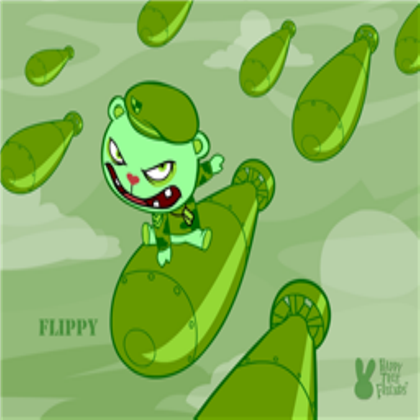
\includegraphics[width=0.6\linewidth]{flippy.png}
\end{figure}

Флиппи сладко спал в своей кровати, когда его внезапно разбудил громкий удар по его домику. Это Гигглс и Каддлс играли в мяч на улице и случайно попали в дом Флиппи. Но так как удар очень 
походил на выстрел из гранатомета, случился флип-аут, а именно проснулся не всеми любимый, добрый и заботливый Флиппи, а злой, жестокий и безжалостный убийца. 
Флиппи-маньяк быстро встал с постели и последовал в гостинную, где была его коллекция огнестрельного оружия. Он выбрал несколько автоматов, но теперь осталось подобрать необходимые пули.
Но открыв коробку с пулями, он обнаружил, что пули различного калибра перепутались и теперь ему необходимо выбрать нужные. Пули, которые подходят для выбранных автоматов, являются простыми числами, то есть их калибр делится только на себя и на 1.
Флиппи достал из подвала специальное пушечное решето - оно помогает фильтровать пули на те, калибр которых является простым числом и на остальные - и стал перебирать заряды.
Через некоторое время все пули были выбраны и Флиппи пошел на свою охоту...

А вы бы смогли отсеять при помощи решета необходимые простые числа до некоторого числа N?

\subsection*{Формат входных данных}
Число N.
\subsection*{Формат выходных данных}
Все простые числа до N, включая его. Каждое число выводится с новой строки.

\newpage


\section*{Задача D. Взрывной пикник}

\begin{tabularx}{\textwidth}{l l X}
    Имя входного файла: & \texttt{\inputFile} \\
    Имя выходного файла: & \texttt{\outputFile} \\
    Ограничение по времени: & $2$ секунды \\
    Ограничение по памяти: & $256$ мегабайт \\
\end{tabularx}

\begin{figure}[h]
	\centering
    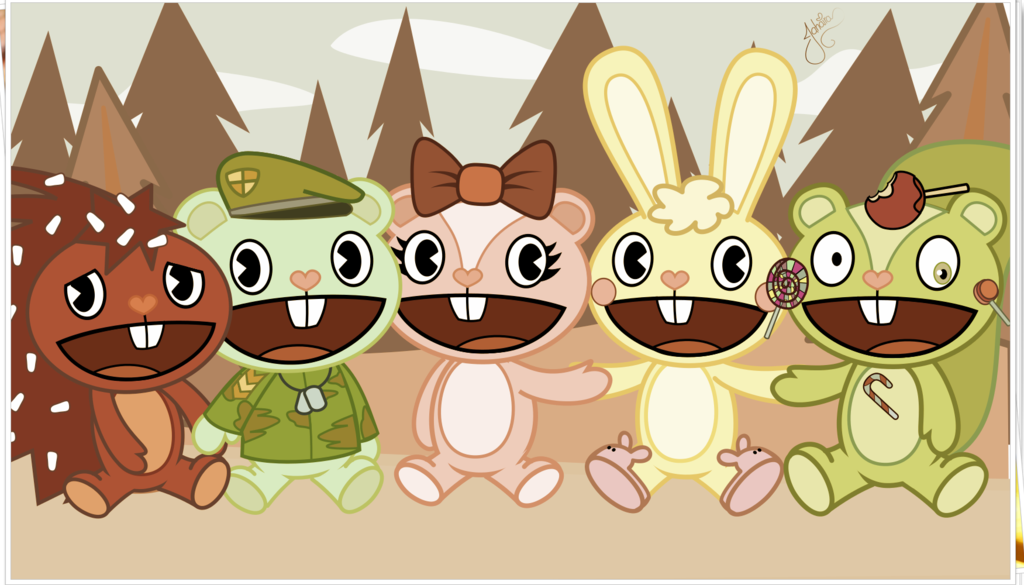
\includegraphics[width=0.5\linewidth]{happy.png}
\end{figure}

Флиппи, Гигглс, Каддлс, Флеки и Натти хотят пойти на пикник, но единственное живописное место --- прекрасная поляна с маленьким прудом, в котором плавают уточки, разноцветными цветами и зеленой мягкой травой
--- не подходит для такого времяпровождения, так как Флиппи в свою последнюю вспышку гнева заминировал чудесную поляну. Для того, чтобы не искать другого места, 
зверята решили попробовать положить плед между минами. Флиппи помнит, что все мины составляют между собой различные треугольники, зверятам необходимо определить треугольник минимального периметра, чтобы точно не попасть на мины во время отдыха.
Флиппи записал на листочке координаты всех мин. Помогите ребятам, определить какие мины составляют минимальный по периметру треугольник, чтобы никто из них не взорвался во время пикника.

\subsection*{Формат входных данных}

Сначала вводится число $N$~---~количество точек ($3 \leq N \leq 50$), а затем $N$ пар вещественных чисел, задающих координаты точек.

\subsection*{Формат выходных данных}

Выведите три числа~---~номера точек, которые должны быть вершинами треугольника, чтобы его периметр был минимален. Если решений несколько выведите любое из них.

\subsection*{Примеры}

\texttt{
    \begin{tabularx}{0.9\textwidth}{| X | X |}
        \hline
        \multicolumn{1}{|c|}{Ввод} & \multicolumn{1}{c|}{Вывод} \\ \hline
        \parbox[t]{\textheight}{
            5 \\
            0 0 \\
            1.3 0 \\
            -2 0.1 \\
            1 0 \\
            10 10 \\
        } & \parbox[t]{\textheight}{
            % Пример вывода. Каждая строчка заканчивается на \\ 
            1 2 4 \\
        } \\ \hline
    \end{tabularx}
}

\newpage


\section*{Задача E. Великаньи спиннеры}

\begin{tabularx}{\textwidth}{l l X}
    Имя входного файла: & \texttt{\inputFile} \\
    Имя выходного файла: & \texttt{\outputFile} \\
    Ограничение по времени: & $2$ секунды \\
    Ограничение по памяти: & $256$ мегабайт \\
\end{tabularx}

\begin{figure}[h]
	\centering
    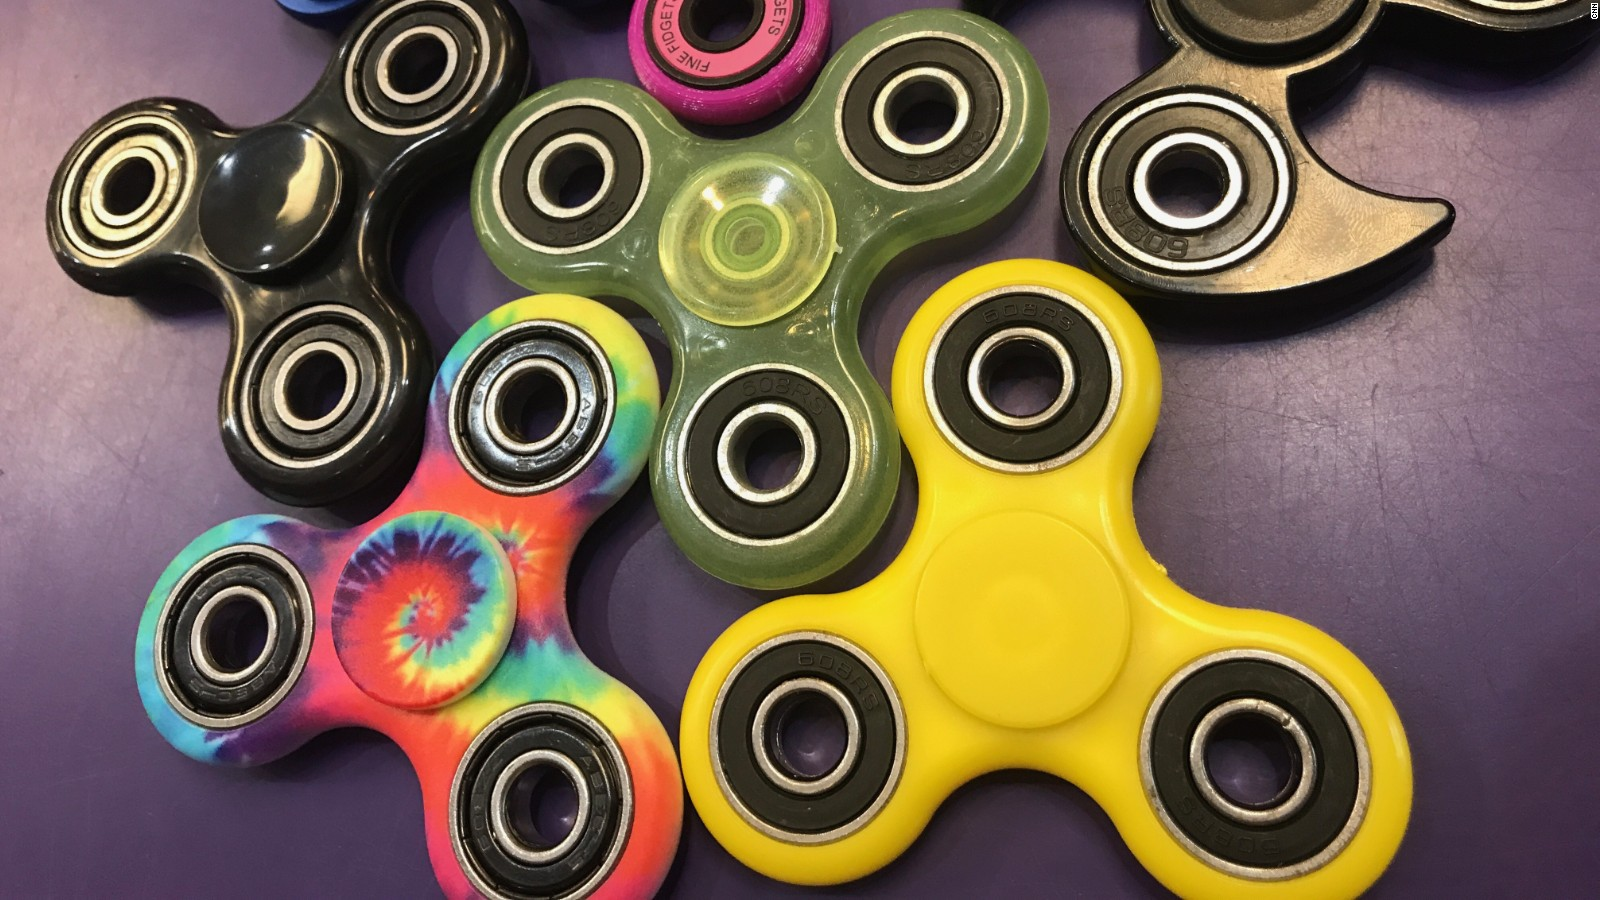
\includegraphics[width=0.6\linewidth]{spinner.jpeg}
\end{figure}

Мальчик-с-пальчик продает спиннеры великанам в Облачном королевстве.
Они весят от 5 до 35 килограмм. Мальчик-с-пальчик хочет продать как можно больше спиннеров (получить как можно больше золотых монет за них), однако его волшебный рюкзак,
который уменьшает все предметы в нем до определенного предела, не всесилен и может принять только ограниченный по весу груз.
Мальчик-с-пальчик отдаст Вам половину вырученной стоимости, если поможете ему с этой задачи.

P.S. Плату спрашивать с Никиты --- он посредник ;)
\subsection*{Формат входных данных}
В первой строке через пробел перечислены общее количество спиннеров ($3 \leq N \leq 20$) и максимальный вес волшебного рюкзака ($3 \leq M \leq 600$) в килограммах.
В следующих $N$ строчках через пробел перечислены стоимость ($N_i$) и вес ($M_i$) отдельно взятого спиннера.
\subsection*{Формат выходных данных}
Вывести одно единственное число --- максимальную стоимость спиннеров без перегруза для Мальчика-с-пальчика.

\subsection*{Примеры}

\texttt{
    \begin{tabularx}{0.9\textwidth}{| X | X |}
        \hline
        \multicolumn{1}{|c|}{Ввод} & \multicolumn{1}{c|}{Вывод} \\ \hline
        \parbox[t]{\textheight}{
            5 13 \\
            1 3 \\
            6 4 \\
            4 5 \\
            7 8 \\
            6 9 \\
        } & \parbox[t]{\textheight}{
            % Пример вывода. Каждая строчка заканчивается на \\ 
            13 \\
        } \\ \hline
    \end{tabularx}
}

\newpage

\end{document}